\chapter{Results} \label{results}

This chapter presents the results of the experiments conducted in the previous chapters. The results are present with an example of execution of a standalone 
module in Optislang.  

\texttt{ARRHENIUS} module is responsible for calculating the field load equivalent testing hours according to Arrhenius lifetime model for each relevant monitor point
in the design. The automation is executed from the file \texttt{main.py} containing the module name and the branch containing the module. 
Code snippet \ref{main_script} provides the code for executing the framework using \texttt{main.py}.

\renewcommand{\lstlistingname}{Code}
\begin{lstlisting}[style=pythoncode, caption={Execution of framework using \texttt{main.py}}, label={main_script}]
from src import ParametricSystem

module_name = "MOO_M_ARRHENIUS"
module_branch_name = 'MOO-1355_py_framework_poc'

def main():
    system = ParametricSystem(module_name, module_branch_name)
    system.clone_module()
    if (
        system.get_module_config_path().exists() & system.get_parameters_path().exists()
    ) == True:
        system.run_module()
        system.verify_output_file()

    else:
        system.json_files_log()

if __name__ == "__main__":
    main()
\end{lstlisting}

\texttt{main.py} calls the \texttt{ParametricSystem} class containing the framework. After cloning the module, the framework verifies the existence of the 
\texttt{\acrshort{json}} files. If the files are not present, the framework provides a log message to the user.

\renewcommand{\lstlistingname}{Code}
\begin{lstlisting}[style=terminal, caption=Error message when \acrshort{json} files are not present, label={json_files_log}]
c:\Users\BIS4SI\Desktop\MOO_Module_Framework\MOO_M_ARRHENIUS\01_Specification\module_config.json does not 
exist 
Please ensure c:\Users\BIS4SI\Desktop\MOO_Module_Framework\MOO_M_ARRHENIUS\01_Specification\module_config.
json exists and re-run
\end{lstlisting}

In code snippet \ref{json_files_log}, the framework provides an error message when the \acrshort{json} file, \texttt{module\_config.json}, is not present.

After verifying the existence of the \acrshort{json} files, the framework continues further to create the required parameters and runs the parametric system.
\begin{figure}[!ht]
    \centering
    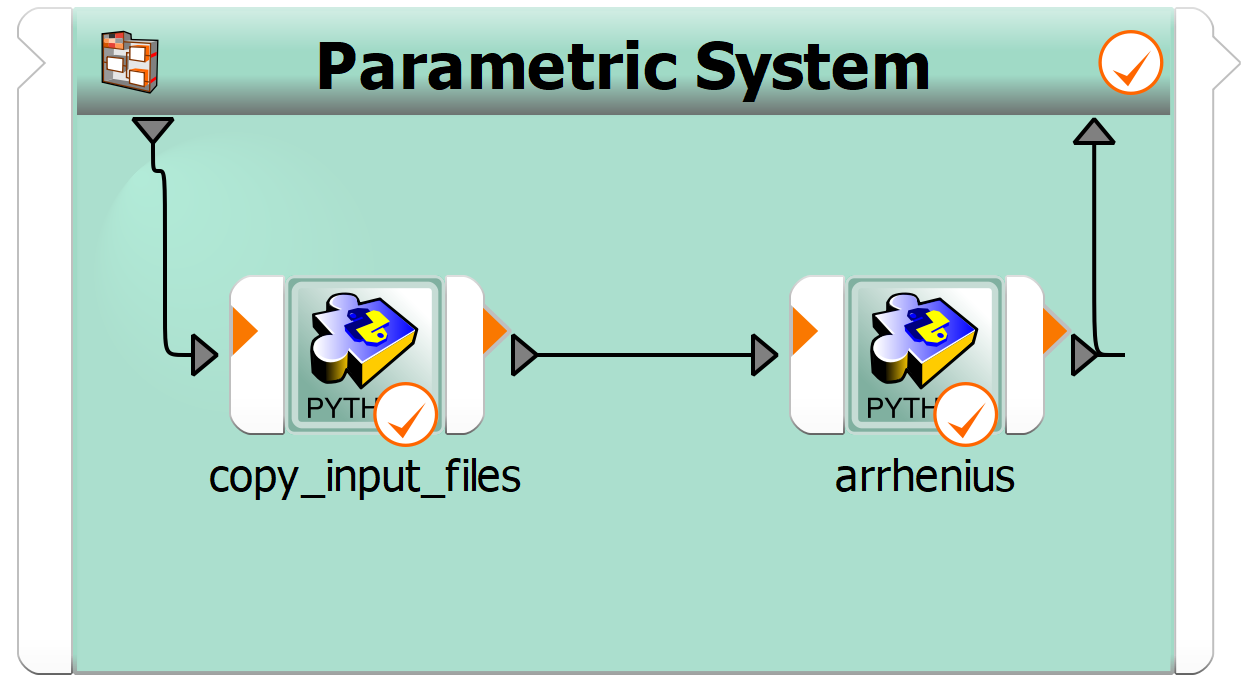
\includegraphics[width=0.5\textwidth]{Images/parametric_system_with_copy_actor.png}
    \caption{Execution of ARRHENIUS module in Optislang}
    \label{parametric_system_with_copy_actor}
  \end{figure}

Figure \ref{parametric_system_with_copy_actor} shows the parametric system created by the framework. The system consists of a python actor, \textbf{copy\_input\_files},
which contains the algorithm to retrieve the input files from OpenShift via \acrshort{api} calls. These input files are stored in the working directory of the 
parametric system. Later, the system continues to run the actor, \texttt{arrhenius}, containing the module. The tick mark on the actors indicate the successful 
execution in Optislang. Successful execution of the parametric system is also displayed in the console as shown in Code snippet \ref{parametric_system_execution}.
\renewcommand{\lstlistingname}{Code}
\begin{lstlisting}[style=terminal, caption=Message providing status of parametric system execution, label={parametric_system_execution}]
Attribute Qt::AA_UseSoftwareOpenGL must be set before QCoreApplication is created.
INFO : Saving project "parametric_system"
INFO : New project "parametric_system". Working dir : "c:\Users\BIS4SI\Desktop\MOO_Module_Framework\MOO_M_
ARRHENIUS\Module\02_Model\parametric_system.opd".
INFO : working directory of "parametric_system" set to "c:\Users\BIS4SI\Desktop\MOO_Module_Framework\MOO_M
_ARRHENIUS\Module\02_Model\parametric_system.opd"
INFO_DETAIL : License feature checkout requested (first of): optislang_level2 [in 281 milliseconds]
INFO_DETAIL : 2024-Sep-30 09:14:07.340325 : License feature checkout requested (first of): optislang_level
2 [in 1 millisecond]
INFO : 2024-Sep-30 09:14:07.340325 : Auto-saving project "parametric_system"
INFO : 2024-Sep-30 09:14:07.409259 : parametric_system : Current iteration successfully prepared
INFO : 2024-Sep-30 09:14:07.409259 : Parametric System : Sent Design 1
INFO : 2024-Sep-30 09:14:07.432607 : Parametric System : Current iteration successfully prepared
INFO : 2024-Sep-30 09:14:11.214374 : copy_input_files : copy_input_files processed successfully [Design 1]
INFO : 2024-Sep-30 09:14:12.848899 : arrhenius : arrhenius processed successfully [Design 1]
INFO : 2024-Sep-30 09:14:12.859403 : Parametric System : Collected Design 1
INFO : 2024-Sep-30 09:14:12.863430 : Parametric System :  Parametric System processed successfully
INFO : 2024-Sep-30 09:14:12.863430 : Auto-saving project "parametric_system"
INFO : 2024-Sep-30 09:14:12.024235 : Auto-saving project "parametric_system"
INFO : 2024-Sep-30 09:14:12.976036 : Auto-saving project "parametric_system"
INFO : 2024-Sep-30 09:14:13.042652 : Total execution time : 6 seconds
INFO : 2024-Sep-30 09:14:13.059409 : Saving project "parametric_system"
\end{lstlisting}

This whole framework is implemented in the \acrshort{ci} pipeline using GitHub Actions. The pipeline is triggered when a developer pushes the code to the 
repository. If all of the steps in the pipeline are successful, new commits are pushed to the branch. If the pipeline fails, the developer is notified via email 
about the failure. This is shown in Figure \ref{github_actions_notification}.
\begin{figure}[!ht]
    \centering
    
\includegraphics[width=0.8\textwidth]{Images/github_actions_notification.png}
    \caption{Notification of pipeline failure in GitHub Actions}
    \label{github_actions_notification}
\end{figure}

After the successful execution of the system in the pipeline, the framework checks the output file generated by the module. Here, the algorithm checks if the
output file generated is as expected, which is provided in \texttt{module\_config.json}. A detailed explanation verification of output files is provided in 
Section \ref{parametric_system_code}. A detailed log message is provided to the user regarding the output file. Code snippet \ref{output_file_verification} shows the log message provided 
to the user. 
\renewcommand{\lstlistingname}{Code}
\begin{lstlisting}[style=terminal, caption={Log message for output file verification}, label={output_file_verification}]
arrhenius_results.csv present
{'monitoring_point': 'str', 'time': 'float'}
Column 'monitoring_point' not found in arrhenius_results.csv
Column 'time' not found in arrhenius_results.csv
\end{lstlisting}
In Code snippet \ref{output_file_verification}, the algorithm confirms the presence of the output file, \texttt{arrhenius\_results.csv}. But, the column names
\texttt{montoring\_point} and \texttt{time} are not present. If the column names are present, it verifies if the data types of the columns are as expected.

The framework is also responsible for creating and excuting MATLAB modules in Optislang. The developer needs to provide the module name and the branch 
name where the module is present. The framework takes care of the rest of the process. Figure \ref{parametric_system_coffin_manson} shows the successful execution of the MATLAB module, 
\texttt{COFFIN MANSON}, in Optislang. 
\newpage
\begin{figure}[!ht]
    \centering
    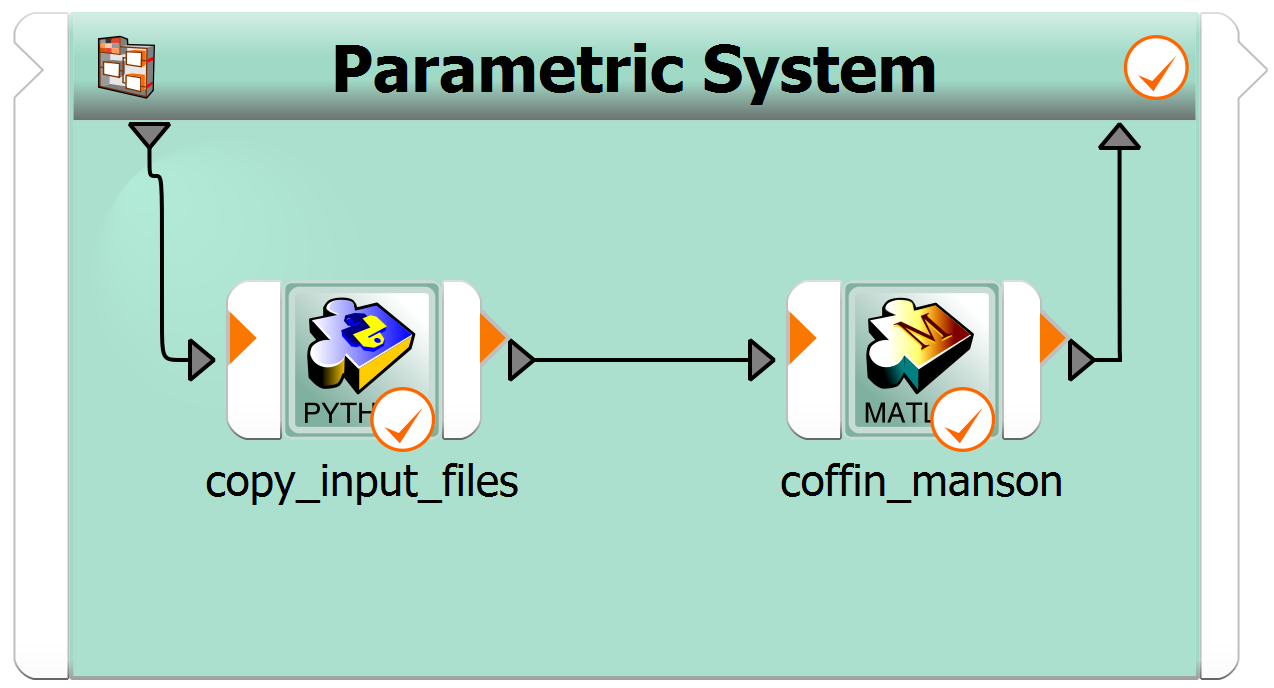
\includegraphics[width=0.5\textwidth]{Images/parametric_system_coffin_manson.png}
    \caption{Execution of MATLAB module in Optislang}
    \label{parametric_system_coffin_manson}
\end{figure}

The execution of the MATLAB modules takes a bit longer compared to the Python module. This is due to execution of MATLAB in the background. 
Currently, the framework is capable of running Python and MATLAB modules. The framework is built in such a way that it can be extended to run other 
modules as well. To run other modules in the framework, the developer only needs to provide the module name and branch of the module. The framework and the 
\acrshort{ci} pipeline take care of the rest of the process.

Earlier, the developer had to manually test their new commits to the module by running the module in Optislang. This process was taking around 30 minutes to 
complete. With the help of the framework, the developer can now run the module in Optislang in seconds. In Code snippet \ref{parametric_system_execution}, the 
framework took around 6 seconds to run the module in Optislang. This is a significant improvement in the time taken to run the module in Optislang compared to the 
manual process. 